\documentclass[a4paper]{article}
\usepackage[left=3.5cm, right=3.5cm, top=2cm]{geometry}
\usepackage{tabularx} 
\renewcommand{\tabularxcolumn}[1]{m{#1}}
\usepackage{graphicx}
\graphicspath{ {./images/} }
\usepackage{multirow}
\renewcommand{\arraystretch}{1.2}

%opening
\title{\textbf{DevOps : Continuous Integration and Continuous Deployment applied} \\~\\
\large \textbf{Project Proposal and Work Plan}}
\author{Hector Pascual Haba}

\begin{document}

\maketitle 

\section{Project overview and goals}
The project is carried out at Silicon Gears an automotive company which works with embedded projects and big build environments that can be automatized in different ways.
\\~\\
The purpose of this project is to research and go deep into the DevOps culture and the trending concepts related to it, which are present in almost each project and company nowadays by designing, developing and implementing a Python tool with some CI and CD features.
\\~\\
The project main goals are:
\begin{itemize}
	\item Get involved with trending DevOps technology.
	\item Get a deep knowledge on DevOps culture and its related concepts.
	\item Develop a CI / CD (Continuous Integration / Continuous Deployment ) tool with features based on other CI tools.
	\item Containerize a build environment and automate its build process as an example.
\end{itemize}


\section{Project background}

This project is conceived as an abstracted wrap up and continuation of all the work I have been doing in the company during last year and also a deep analysis of concepts related to DevOps culture that I have got to learn in order to proceed. With abstracted I mean that no confidential data will be present on any document. The only way I will be using all the work done internally in the company is as base knowledge to develop this project.
\\~\\
The project itself will be independent on company projects due to the abstraction performed. 
The main project ideas are completely provided by the author nor the supervisor.

\section{Project requirements and specifications}

The focus of this section will be mainly oriented to the tool that I will be developing along the thesis, due to its practical approach.
\\~\\
Project requirements:
\begin{itemize}
	\item The project should cover all the DevOps related concepts described in the sections.
	\item The project should contain reflections on different ways to perform automation of processes.
	\item The tool should be able to automatize any process that can be done manually via shell commands.
	\item The tool should be able to schedule jobs periodically through cron expressions.
	\item The tool should be able to describe the processes to automatize through pipelines.
\end{itemize}
Project specifications:
\begin{itemize}
	\item Each concept not explained previously related to DevOps must have a reference to an article or book that quotes it.
	\item The project should contain technical examples when an automation process is described (i.e: Wrapping up a build environment with Docker and deploying it with Ansible to multiple physical hosts.)
	\item The tool should be able to be hosted on Linux system connected to a private network.
	\item The tool should be accessible through a REST API developed on Python.
	\item The Python version used on development should be at least Python 3.6.
	
\end{itemize}
\section{Work Plan}
\subsection{Work Breakdown Structure}
~\\~\\
\begin{figure}[h]
	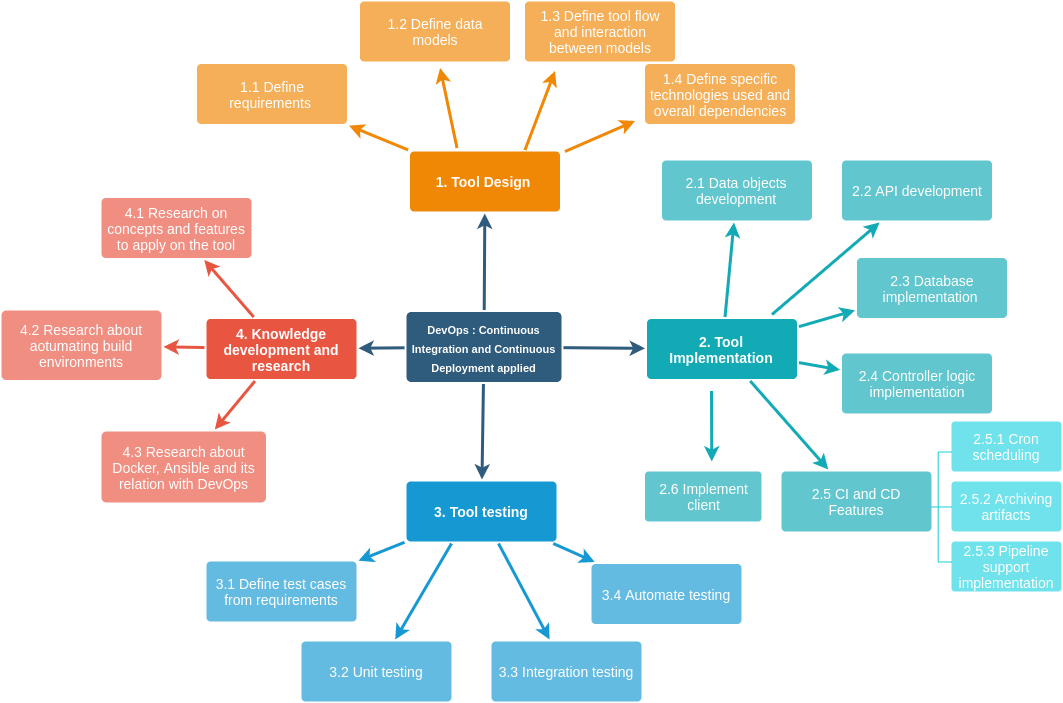
\includegraphics[scale=0.4]{wp_breakdown}
\end{figure}
\newpage
\subsection{Work Packages, Tasks and Milestones}
~\\
\begin{tabularx}{\textwidth}{|X|c|}
	\hline
	\textbf{WP Name:} Define requirements& \textbf{WP ref: 1.1} \\ \hline
	\textbf{Major constituent:} Tool Design & - \\ \hline
	\multirow{2}{*}{\begin{tabular}[c]{@{}l@{}}\textbf{Short description:} Define specific requirements\\based on DevOps real world culture and concepts \end{tabular}} &  \textbf{Planned start date:} 16/Feb/2020\\ \cline{2-2} 
	&  \textbf{Planned end date:} 19/Feb/2020\\ \hline
\end{tabularx}
\\\vspace{5px}\\
\begin{tabularx}{\textwidth}{|X|c|}
	\hline
	\textbf{WP Name:} Define data models& \textbf{WP ref: 1.2} \\ \hline
	\textbf{Major constituent:} Tool Design & - \\ \hline
	\multirow{2}{*}{\begin{tabular}[c]{@{}l@{}}\textbf{Short description:} Think about data models\\that will define the tool and its DB representation. \end{tabular}} &  \textbf{Planned start date:} 24/Feb/2020\\ \cline{2-2} 
	&  \textbf{Planned end date:} 26/Feb/2020\\ \hline
\end{tabularx}
\\\vspace{5px}\\
\begin{tabularx}{\textwidth}{|X|c|}
	\hline
	\textbf{WP Name:} Define tool flow and interaction& \textbf{WP ref: 1.3} \\ \hline
	\textbf{Major constituent:} Tool Design & - \\ \hline
	\multirow{2}{*}{\begin{tabular}[c]{@{}l@{}}\textbf{Short description:} Define the application flow\\of the application and how the models will\\interact between them.  \end{tabular}} &  \textbf{Planned start date:} 26/Feb/2020\\ \cline{2-2} 
	& \multicolumn{1}{c|}{\begin{tabular}[c]{@{}c@{}}\\\textbf{Planned end date:} 27/Feb/2020\end{tabular}}\\ & \\ \hline
\end{tabularx}
\\\vspace{5px}\\
\begin{tabularx}{\textwidth}{|X|c|}
	\hline
	\textbf{WP Name:} Define specific technologies and dependencies& \textbf{WP ref: 1.4} \\ \hline
	\textbf{Major constituent:} Tool Design & - \\ \hline
	\multirow{2}{*}{\begin{tabular}[c]{@{}l@{}}\textbf{Short description:} Define programming\\languages involved, general dependencies and\\technologies that will be used. \end{tabular}} &  \textbf{Planned start date:} 25/Feb/2020\\ \cline{2-2} 
	& \multicolumn{1}{c|}{\begin{tabular}[c]{@{}c@{}}\\\textbf{Planned end date:} 25/Feb/2020\end{tabular}} \\ 
	& \\ \hline
\end{tabularx}
\\\vspace{5px}\\
\begin{tabularx}{\textwidth}{|X|c|}
	\hline
	\textbf{WP Name:} Data objects development& \textbf{WP ref: 2.1} \\ \hline
	\textbf{Major constituent:} Tool Implementation & - \\ \hline
	\multirow{2}{*}{\begin{tabular}[c]{@{}l@{}}\textbf{Short description:} Represent the data models\\in Python class and the database models as well. \end{tabular}} &  \textbf{Planned start date:} 02/Mar/2020\\ \cline{2-2} 
	&  \textbf{Planned end date:} 05/Mar/2020\\ \hline
\end{tabularx}
\\\vspace{5px}\\
\begin{tabularx}{\textwidth}{|X|c|}
	\hline
	\textbf{WP Name:} API Developments& \textbf{WP ref: 2.2} \\ \hline
	\textbf{Major constituent:} Tool Implementation & - \\ \hline
	\multirow{2}{*}{\begin{tabular}[c]{@{}l@{}}\textbf{Short description:} Development of the API in\\order to make the models accessible from a client. \end{tabular}} &  \textbf{Planned start date:} 09/Mar/2020\\ \cline{2-2} 
	&  \textbf{Planned end date:} 24/Mar/2020\\ \hline
\end{tabularx}
\\\vspace{5px}\\
\begin{tabularx}{\textwidth}{|X|c|}
	\hline
	\textbf{WP Name:} Database Implementation& \textbf{WP ref: 2.3} \\ \hline
	\textbf{Major constituent:} Tool Implementation & - \\ \hline
	\multirow{2}{*}{\begin{tabular}[c]{@{}l@{}}\textbf{Short description:} Implement the logic for\\accessing to the SQL database using Python. \end{tabular}} &  \textbf{Planned start date:} 03/Mar/2020\\ \cline{2-2} 
	&  \textbf{Planned end date:} 10/Mar/2020\\ \hline
\end{tabularx}
\\\vspace{5px}\\
\begin{tabularx}{\textwidth}{|X|c|}
	\hline
	\textbf{WP Name:} Controller logic implementation& \textbf{WP ref: 2.4} \\ \hline
	\textbf{Major constituent:} Tool Implementation & - \\ \hline
	\multirow{3}{*}{\begin{tabular}[c]{@{}l@{}}\textbf{Short description:} Develop the logic for using\\the data models and giving capabilities for user\\interaction through the API.\end{tabular}} &  \textbf{Planned start date:} 08/Mar/2020\\ \cline{2-2} 
	& \multicolumn{1}{c|}{\begin{tabular}[c]{@{}c@{}}\\\textbf{Planned end date:} 29/Mar/2020\end{tabular}}\\ 
	&  \\ \hline
\end{tabularx}
\\\vspace{5px}\\
\begin{tabularx}{\textwidth}{|X|c|}
	\hline
	\textbf{WP Name:} CI and CD Features& \textbf{WP ref: 2.5} \\ \hline
	\textbf{Major constituent:} Tool Design & - \\ \hline
	\multirow{2}{*}{\begin{tabular}[c]{@{}l@{}}\textbf{Short description:} Basing on the research done\\in parallel in WP 4.1 implement features. \end{tabular}} &  \textbf{Planned start date:} 30/Mar/2020\\ \cline{2-2} 
	&  \textbf{Planned end date:} 22/Apr/2020\\ \hline
	\multicolumn{2}{|l|}{\begin{tabular}[c]{@{}l@{}}\textbf{2.5.1 Cron scheduling}: Implementing capability to  schedule jobs periodically with \\ cron expressions\end{tabular}} \\ \hline
	\multicolumn{2}{|l|}{\begin{tabular}[c]{@{}l@{}}\textbf{2.5.2 Archiving artifacts}: Implementing capability to store binaries and outputs\\from build executions\end{tabular}} \\ \hline
	\multicolumn{2}{|l|}{\begin{tabular}[c]{@{}l@{}}\textbf{2.5.3 Pipeline support}: Implementing capability to define builds through YAML \\pipelines.\end{tabular}} \\ \hline
\end{tabularx}
\\\vspace{5px}\\
\begin{tabularx}{\textwidth}{|X|c|}
	\hline
	\textbf{WP Name:} Implement Client& \textbf{WP ref: 2.6} \\ \hline
	\textbf{Major constituent:} Tool Implementation & - \\ \hline
	\multirow{2}{*}{\begin{tabular}[c]{@{}l@{}}\textbf{Short description:} Implement a client with GUI\\in order to interact with the API.\end{tabular}} &  \textbf{Planned start date:}24/Apr/2020\\ \cline{2-2} 
	&  \textbf{Planned end date:} 20/May/2020\\ \hline
\end{tabularx}
\\\vspace{5px}\\
\begin{tabularx}{\textwidth}{|X|c|}
	\hline
	\textbf{WP Name:} Define test cases from requirements& \textbf{WP ref: 3.1} \\ \hline
	\textbf{Major constituent:} Tool Testing & - \\ \hline
	\multirow{2}{*}{\begin{tabular}[c]{@{}l@{}}\textbf{Short description:} Define test cases based on\\the requirements defined on WP 1.1 \end{tabular}} &  \textbf{Planned start date:} 21/May/2020\\ \cline{2-2} 
	&  \textbf{Planned end date:} 25/May/2020\\ \hline
\end{tabularx}
\\\vspace{5px}\\
\begin{tabularx}{\textwidth}{|X|c|}
	\hline
	\textbf{WP Name:} Unit tests& \textbf{WP ref: 3.2} \\ \hline
	\textbf{Major constituent:} Tool Testing & - \\ \hline
	\multirow{2}{*}{\begin{tabular}[c]{@{}l@{}}\textbf{Short description:} Write unit tests for each\\module and function that is critical. \end{tabular}} &  \textbf{Planned start date:} 25/May/2020\\ \cline{2-2} 
	&  \textbf{Planned end date:} 27/May/2020\\ \hline
\end{tabularx}
\\\vspace{5px}\\
\begin{tabularx}{\textwidth}{|X|c|}
	\hline
	\textbf{WP Name:} Integration Testing& \textbf{WP ref: 3.3} \\ \hline
	\textbf{Major constituent:} Tool Testing & - \\ \hline
	\multirow{2}{*}{\begin{tabular}[c]{@{}l@{}}\textbf{Short description:} Write integration tests\\checking overall tool functionality. \end{tabular}} &  \textbf{Planned start date:} 27/May/2020\\ \cline{2-2} 
	&  \textbf{Planned end date:} 29/May/2020\\ \hline
\end{tabularx}
\\\vspace{5px}\\
\begin{tabularx}{\textwidth}{|X|c|}
	\hline
	\textbf{WP Name:} Automate testing& \textbf{WP ref: 3.4} \\ \hline
	\textbf{Major constituent:} Tool Testing & - \\ \hline
	\multirow{2}{*}{\begin{tabular}[c]{@{}l@{}}\textbf{Short description:} Automate testing to be\\executed when merges to master are done. \end{tabular}} &  \textbf{Planned start date:} 01/Jun/2020\\ \cline{2-2} 
	&  \textbf{Planned end date:} 04/Jun/2020\\ \hline
\end{tabularx}
\\\vspace{5px}\\
\begin{tabularx}{\textwidth}{|X|c|}
	\hline
	\textbf{WP Name:} Research on concepts and features to apply on the tool& \textbf{WP ref: 4.1} \\ \hline
	\textbf{Major constituent:} Knowledge development and research & - \\ \hline
	\multirow{2}{*}{\begin{tabular}[c]{@{}l@{}}\textbf{Short description:} Read books and articles\\trending on the topic to conclude features that \\ might fit on the tool. \end{tabular}} &  \textbf{Planned start date:} 10/Mar/2020\\ \cline{2-2} 
	&  \multicolumn{1}{c|}{\begin{tabular}[c]{@{}c@{}}\\\textbf{Planned end date:} 04/Jun/2020\end{tabular}} \\
	& \\ \hline
\end{tabularx}
\\\vspace{5px}\\
\begin{tabularx}{\textwidth}{|X|c|}
	\hline
	\textbf{WP Name:} Research about automating build environments & \textbf{WP ref: 4.2} \\ \hline
	\textbf{Major constituent:} Knowledge development and research & - \\ \hline
	\multirow{2}{*}{\begin{tabular}[c]{@{}l@{}}\textbf{Short description:} Strictly related to 4.3, get\\conclusions on this topic and write thoughts. \end{tabular}} &  \textbf{Planned start date:} 11/May/2020\\ \cline{2-2} 
	&  \multicolumn{1}{c|}{\begin{tabular}[c]{@{}c@{}}\\\textbf{Planned end date:}
			01/Jun/2020\end{tabular}}\\ 
	& \\\hline
\end{tabularx}
\\\vspace{5px}\\
\begin{tabularx}{\textwidth}{|X|c|}
	\hline
	\textbf{WP Name:} Research about Docker, Ansible and its relation with DevOps& \textbf{WP ref: 4.3} \\ \hline
	\textbf{Major constituent:} Knowledge development and research & - \\ \hline
	\multirow{2}{*}{\begin{tabular}[c]{@{}l@{}}\textbf{Short description:} Research and write ways in\\which these technologies can be used and applied. \end{tabular}} & \textbf{Planned start date:} 14/May/2020\\ \cline{2-2} 
	&  \textbf{Planned end date:} 02/Jul/2020\\ \hline
\end{tabularx}

\subsection{Time Plan (Gantt diagram)}

\begin{figure}[h]
	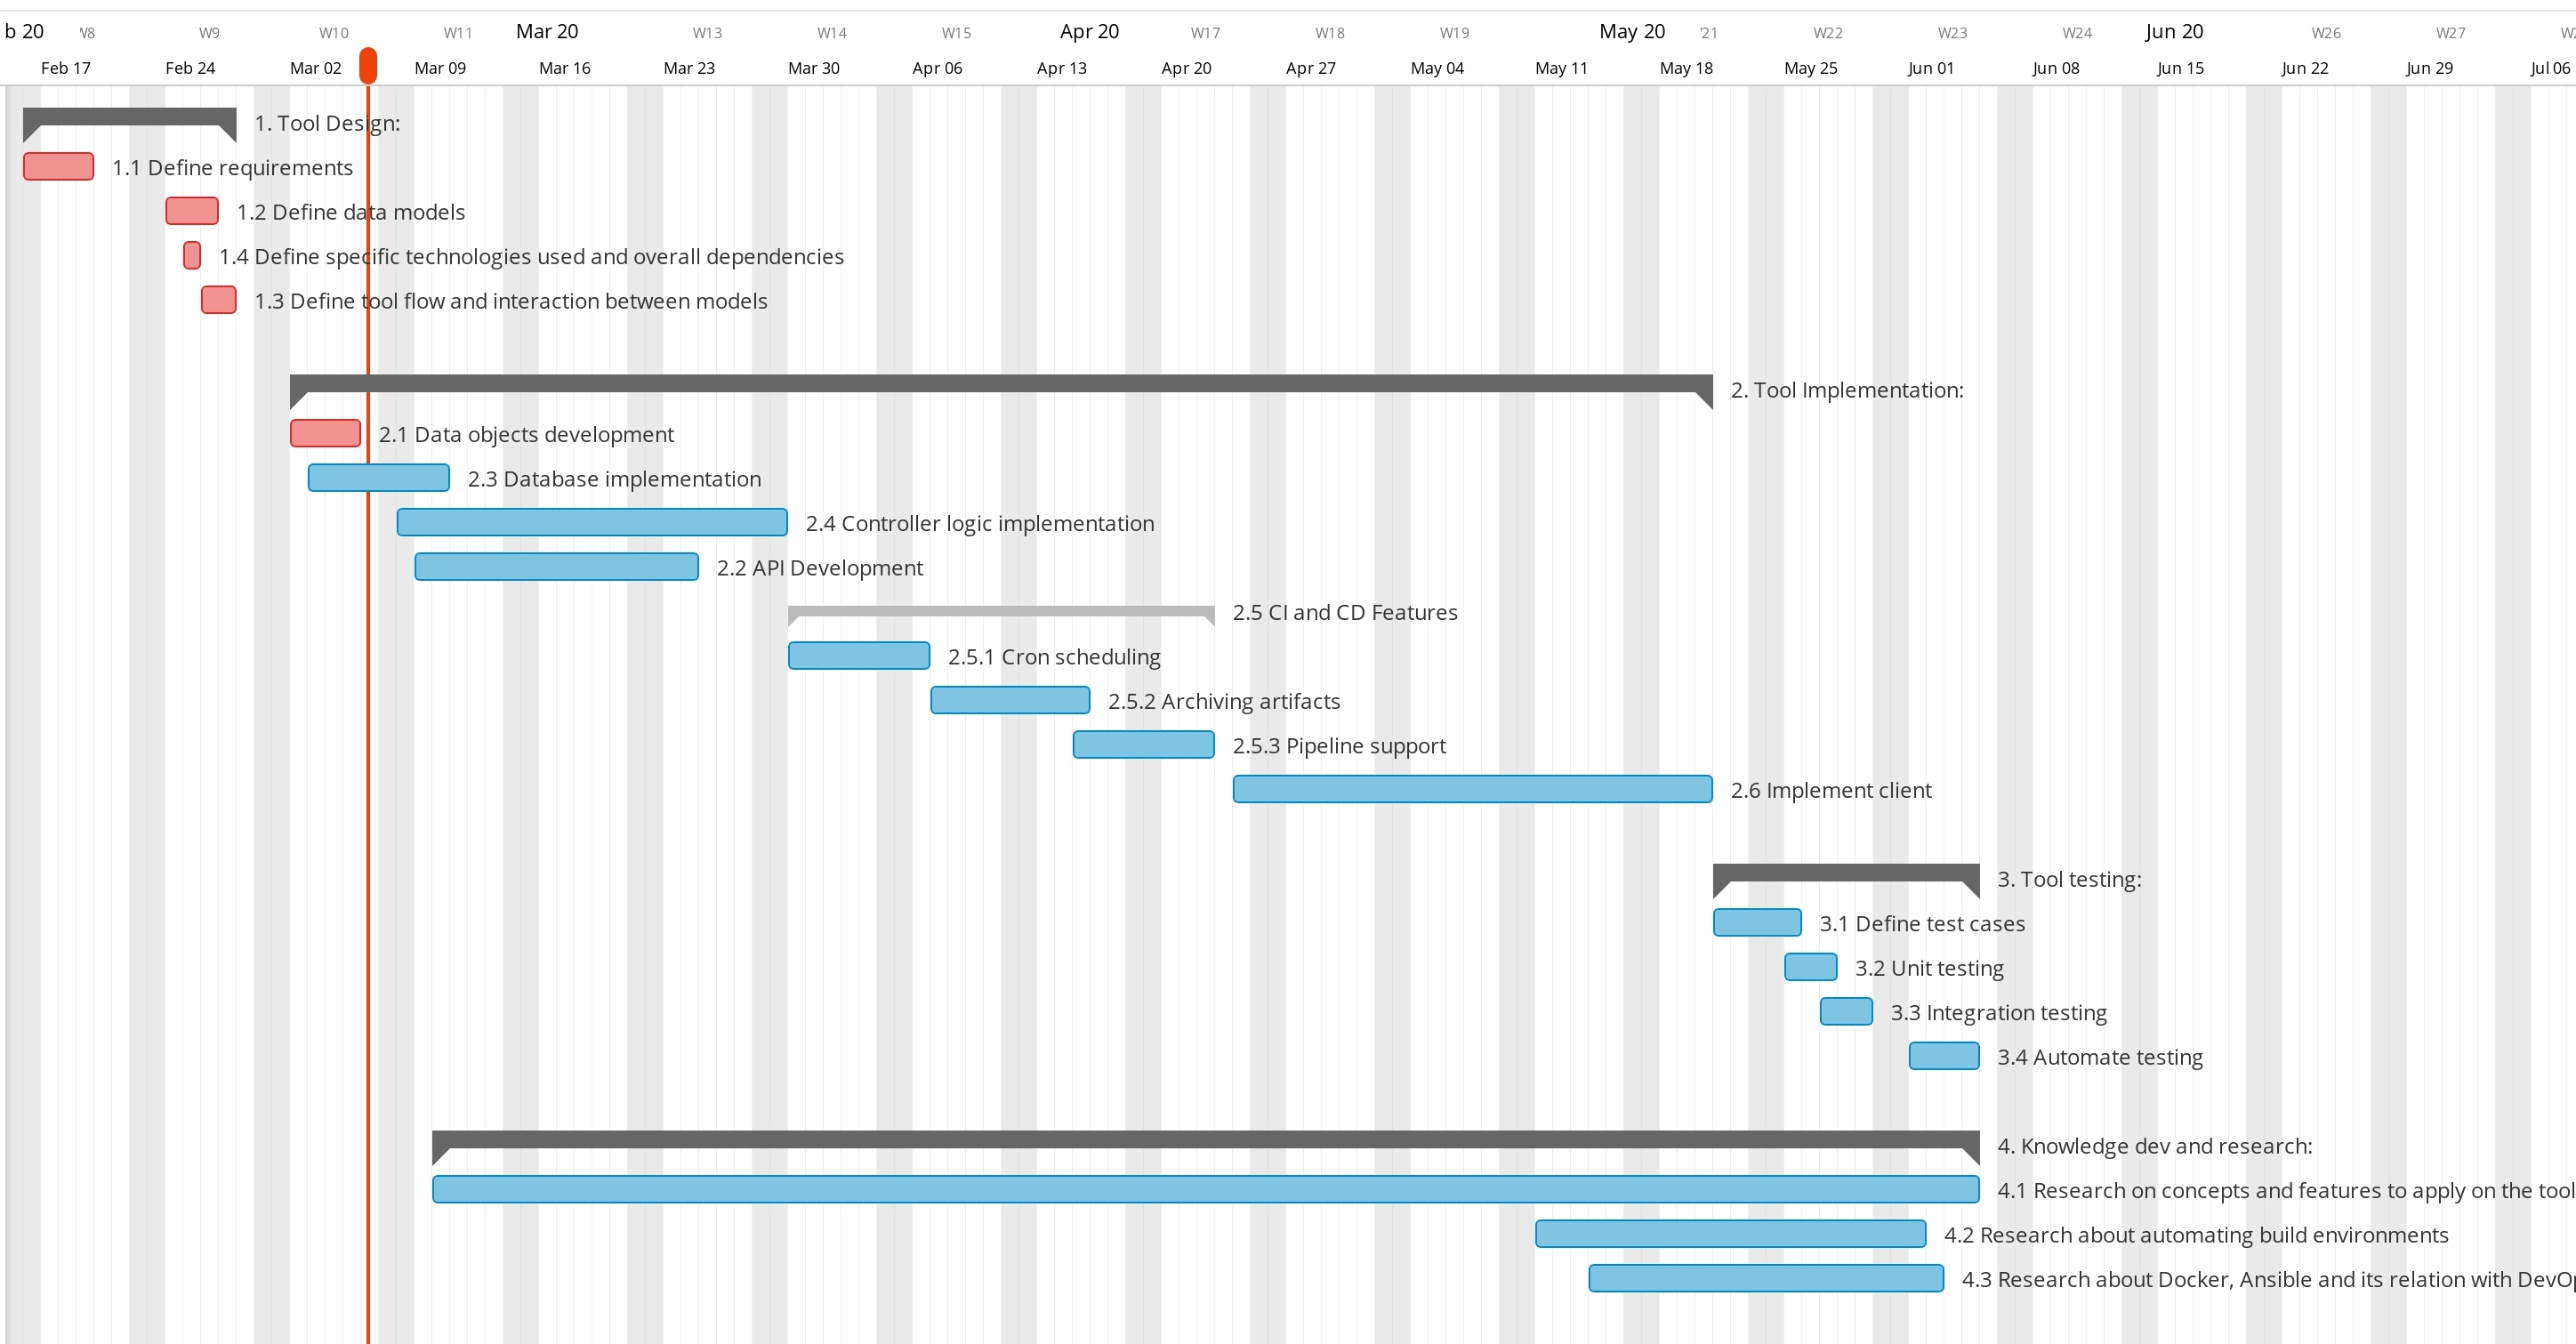
\includegraphics[scale=0.12]{gantt}
\end{figure}
\newpage
\section{Generic skills}

The generic skills that will be worked intensively while carrying the project out will be the following :
\\~\\
\begin{tabularx}{\textwidth}{|c|X|X|}
	\hline
	\textbf{\#} & \textbf{Generic Skill} & \textbf{Explanation} \\ \hline
	1  & Oral and written communication & Written up of the project and oral presentations.\\ \hline
	2  & Autonomous learning. & In order to carry out the project I got to design solutions that use current trending technologies which I had to learn by myself. \\ \hline
	3  & Ability to identify, formulate and solve engineering problems & Automating manual processes requires an ability to identify step by step what is being done, formulate an automation proposal and design a solution.  \\ \hline
	4  & Ability to Conceive, Design, Implement and Operate complex systems in the ICT context & The design and implementation of the CI/CD tool requires to be highly capable of the skill mentioned.
	     \\ \hline
\end{tabularx}




\end{document}
